% !TEX root = ../report.tex


\section{In-vehicle Communication Networks and Security}\label{sec:communication-networks}

The different functions of a vehicle have very different requirements in
performance and safety needs. Therefor the quality of service needed from the
communication system varies (e.g.\ response time or bandwidth). Normally there
are different functional domains which divide the in-car embeeded
systems~\cite{Navet2017}. There are the safety-critical domains ``powertrain''
(e.g. engine control) and ``chassis'' (e.g.\ steering) that need a deterministic
real-time behavior. The functions of the ``body'' domain that controls for
example dashboard, wipers, lights and windows need to exchange many informations
of small size between each other. Other domains like ``telematics'' and
``multimedia'' have for example increased requirements in bandwidth and
confidentiality.

A multitude of different networks resulted out of this diversity of
requirements. Therefor the Society of Automotive Engineers (SAE) created in 1994
a classification for automotive communication protocols. This classification is
based on data transmision speed and functionality. There were 4 different
classes defined that are labeled class A to class D~\cite{Ali2017}. Class A
networks have a speed lower than 10 kb/s. They are used for convenience features
such as trunk release or electric mirror adjustment. Examples for Class A
networks are LIN and TTP/A. Class B has a medium speed of 10 to 125~kb/s.
Networks of this classification are for general information between ECUs from
for example sensors. Main representatives of this class are J1850 and low-speed
CAN\@. High speed networks of class C have a speed between 125~kb/s and 1 Mb/s and
are used for real time control like the power train or vehicle dynamics.
High-speed CAN falls into this classification. Above the high speed
classification C there is class D\@. Every communication protocol faster than 1
Mb/s fall into this category. They are normally used either for multimedia
applications (e.g. MOST) or for hard real time critical functions like X-by-Wire
applications (e.g. TTP/C or FlexRay). Networks this fast, like FlexRay, can also
be used as gateways between sub-systems.

In modern vehicles it is normal that there are many networks of different types.
A BMW 7 series car from 2008 implements for example multiple LIN buses, a MOST
and a FlexRay bus and additionally four CAN buses~\cite{Kellermann2008}. All of
these networks are normally interconnected by gateways.

In-vehicle networks play a crucial role in keeping the embedded systems in a
safe state. Depending on the network it can be for example more or less
difficult to identify failed nodes. Also some networks can meet hard real-time
constraints and some cannot. In general there are two main paradigms in
automotive communication, event-triggered and time-triggered communication
\cite{Navet2017}. If the communication is consisting of asynchronous events, it
follows the event-triggered paradigm. In such systems it is crucial to avoid
conflicts while sending events from multiple sources in parallel.
Event-triggered systems use the bandwidth effectively and are easy to extend
with new network nodes. If network communication is synchronous, so every nodes
sends at predefined time slot in a defined interval, then the communication
follows the time-triggered paradigm. In general accessing a medium this way is
called Time Division Multiple Access (TDMA). These systems are perfectly
predictable but require to be statically defined up front. If there are new
nodes introduced to the network the schedule has to be changed, so it is more
complicated to extend these systems. Also the bandwidth is not used very
efficiently and the response times are longer then in event-triggered systems.
However missing messages can be identified rather easily. Because both paradigms
have up and down sides. Normally both types of communications are needed for
different features in an embedded system of a vehicle. Hence some networks like
FlexRay provide both types of communication alongside each other.

In the following sub-chapters I will describe the CAN network and give an
overview about some of the most representative other networks.

\subsection{CAN Network}

The CAN network was introduced in 1983 by the Robert Bosh GmbH~\cite{Navet2017}.
It uses a twisted pair of copper wires as a bus between the nodes. Depending on
the speed used it is either classified and used as a SAE class B or class C
network. Aside the used speed there are two versions of CAN\@. Version 2.0A and
2.0B which differ in the length of the identifier used when sending data. CAN
uses a Non-Return-to-Zero bit representation with a bit stuffing of 5~bits.
Which means the bits will be represented by continuous levels of voltage. To be
able to stay in sync when sequences of the same bit value are sent over the wire
there will be the other bit value ``stuffed'' in after every 5 same consecutive
values. The receivers know this and can properly ``destuff'' the bit sequence.
So all CAN nodes can stay in sync using this bit stuffing. 

For CAN to be able to bound the respond times it uses a priority system. The
lower the identifier used to send data the higher the priority. To realize these
priorities the physical layer needs to implement an ``AND'' scheme. Only when
everyone simultaneously sends a 1 the resulting bus level is 1. If one node on
the bus sends a 0, the resulting bus level has to be a 0. So the 0 is the
dominant value on the bus and overrides a 1. With this mechanism it is easy to
realize the priority system.

The normally used version of CAN is 2.0A because it provides with \(2^{11}\)
possibilities enough identifiers so I will focus on its specs in the following.
Communication over the CAN bus is organized into frames of a maximum size of
135~bits if all overheads are included. A frame starts with a 1~bit Start Of
Frame. Following this start there is an 18~bit header. The header contains the
11~bit identifier, the Remote Transmission Request~(RTR) bit and the Data Length
Code~(DLC). The RTR distinguished between data frames and data request frames.
The DLC provides the length of the data following after the header. This data
can have at most 8~bytes. After the data follows a 15~bit Cyclic Redundancy
Check (CRC) for ensuring data integrity. After the CRC follows the
Acknowledgement field (Ack). With the Ack a sender is possible to know that a
sender has received the frame. However it is not possible to distinguish who
received it. At the end of the frame is the End Of Frame field followed by the
intermission bits. The intermission bits are the minimal number of bits after
which it is allowed to send a new data frame.

TODO\@: image of data frame composition

On an idle CAN bus every node can send a data frame at any time. If multiple
nodes want to send a frame simultaneously and collide the priority based
arbitration decides which node is allowed to send data. This works with the help
of the physical layer implementing the ``AND'' scheme. So while sending
identifier and RTR bit the nodes are observing the bus level. If the node
observes a bit of its own to be overridden by a dominant bit (0 is dominant over
1) it stops sending data because another node with a smaller identifier plus RTR
is sending at the same moment which has priority. The node which stopped sending
needs to wait until the bus becomes idle again and then tries to send the data
frame again.

For the priority-based arbitration to work the signal of a bit needs to
propagate to all other nodes and back before sending the next bit. So the
physical length of the bus restricts the speed with which data can be send. On a
40 meter bus a maximum speed of 1 Mbit/s is possible while only 250 Kbit/s can
be achieved over a 250 meter long bus~\cite{Navet2017}. This restriction has
lead to optimizations by the car manufacturers using ``traffic shaping''. One
example would be to use an offset for important periodic messages so they will
not interfere with each other~\cite{Navet2009}

The CAN protocol has different mechanisms to detect possible errors. One
mechanism would be to use the CRC to validate the data integrity. If an error is
detected by a node it will send six consecutive dominant bits which will cancel
the current data frame. This will alert all nodes on the bus that an error
occurred and a new arbitration phase can start. This delays the message sending
and possible deadlines may be missed this way. The possible start of a new frame
takes 17 to 31~bits after an error was detected. CAN also includes some
fault-confinement mechanisms for failures for example on the hardware level of
the micro-controller or communication controller. These mechanisms normally
involve the counting of failures and successful delivery of frames. However each
node is responsible itself to execute these mechanisms. So the relevance of
these mechanisms is questionable~\cite{Navet2017}. If there is an error for
example with the oscilloscope a node could be sending unknowingly many dominant
bits. This would be one manifestation of the ``babbling
idiot''~\cite{Pimentel2009}. More mechanisms are needed if the protocol is used
for safety-critical functions. There are lots of different solutions for
different problems but there is no formal verification for these mechanisms used
together~\cite{Navet2017}.

The CAN protocol only defines the physical layer and the Data Link layer but
there are higher level protocols like AUTOSAR which use the CAN protocol.

\subsection{Other Representative Networks}

There are other priority bus systems besides CAN like J1850 and VAN but they are
used less and less in favor of CAN~\cite{Navet2017}. In 2012 Robert Bosch GmbH
introduced a new CAN version named CAN FD~\cite{Hartwich2012}. It distinguishes
itself from standard CAN through higher data rates outside of the arbitration
phase and the possibility for larger data fields. Another advantage is the easy
migration from CAN to CAN FD because only the underlying communication layer has
to be changed. The nodes using CAN can remain unchanged.

Event-triggered networks such as CAN are not suited for all use cases of IVNs.
Event-triggered systems have lightweight protocols with dynamic arbitration per
message and good use of bandwidth. However they are hard to verify formally in
regard to e.g.\ bounded response times. If deterministic real time behavior is
needed for e.g.\ X-by-Wire Systems, it is more suitable to choose a
time-triggered network based on TDMA~(Time Division Multiple Access). They have
protocols with static arbitration and need a clock synchronization. The two TDMA
based networks suitable for serving as a gateway between IVNs or as a basis for
safety critical applications in vehicles are FlexRay and
TTEthernet~\cite{Navet2017}. 

The FlexRay specification was initially created by the FlexRay consortium which
was an alliance of car manufacturers, semiconductor and electronic systems
manufacturers (established in 2000). FlexRay is a very flexible network aiming
to provide advantages from the time-triggered and the event-driven world by
integrating both schemes into one protocol. It is possible to scale the ratio
between the time-triggered and the event-driven part of the protocol for
adapting the network to the use case. Theoretically it is possible to use just
one part of the protocol, the event-driven or time-triggered one.

Besides high speed and real time requirements, there are also parts of the
in-vehicle networks with very few requirements in comparison. Their primary
requirement is to have low costs. There are a multitude of such networks. The
Local Interconnect Network (LIN) and TTP/A are two representatives of these
networks whereupon TTP/A is not used in production vehicles and very similar to
LIN~\cite{Navet2017}, so I will not go into detail about TTP/A. Low-cost
automotive networks are normally used to control seats, doors, etc. They are not
only cheap because of the simple communication protocol but also because of the
low requirements in regard to micro-controller hardware. LIN is a master/slave
network with a single master node polling all the slave nodes for information.
The slave nodes are not allowed to initiate communication. Also LIN is able to
send nodes to sleep and to wake them up which is very important in the
automotive context. It works with just a single copper cable with a data rate up
to 20Kbit/s.

The third big IVN domain in vehicles is multimedia and infotainment networks.
The de-facto standard in this domain is the Media Oriented System Transport
(MOST)~\cite{Navet2017} developed by the MOST Coorporation~\cite{MOST2018} which
is a consortium of car manufacturers and suppliers. MOST uses Polymer Optical
Fiber or coaxial transmission as the physical layer. It integrates the
possibility to transport standard ethernet frames. So it is possible to
transport content and information for example from the web. The current MOST
provides speed up to 150~Mbit/s. However the MOST Coorporation is working on a
new version with speed up to 5~Gbit/s to be able to contend with automotive
ethernet which is an upcoming competitor.

Today, automotive ethernet is named as the future of in-vehicle networks.
However it has still not oust its competitors. Though in 2022 it is likely that
there are more ethernet ports inside of vehicles than anywhere
else~\cite{Ixia2014}. There are two major representatives of automotive ethernet
networks which are Ethernet Audio/Video Bridging (AVB) and TTEthernet. Ethernet
AVB works with over-provisioning and prioritisation while the FlexRay competitor
TTEthernet is a time-triggered switched ethernet protocol utilizing TDMA\@.
TTEthernet provides mixed-criticality temporal requirements. It describes three
types of traffic streams with upper bounds on latency and jitter for two of the
three types. TTEthernet was designed for the most critical use-cases even
including aeronautic applications. Ethernet AVB was designed for low-latency
streaming services over ethernet by a consortium of car manufacturers and
suppliers called AVnu Alliance~\cite{AVNU2018}.

Automotive ethernet also needs some adjustments of the physical layer to work
properly in the vehicular environment in regard to cost, power saving modes,
robustness to environmental condition, etc. A physical ethernet layer developed
by the OPEN Alliance SIG~\cite{SIG2018} for the vehicular environment is
BroadR-Reach. It uses low cost unshielded copper wires. 

\subsection{Security Measures}

In-vehicle communication needs to be secured end-to-end so that no one else than
the intended receiver can read the messages, no one is able to modify message
content unnoticed and unauthorized parties are not able to participate in the
communication~\cite{Lemke2006}. There are three elementary security practices
for achieving security in IVN communication. The following report focuses on the
first elementary practice: Controller Authentication.

\subsubsection{Controller Authentication}

Every valid controller sending messages in the IVN needs to be authenticated. So
that it is possible to distinguish messages from unauthorized parties and to be
able to process these separately or just discard them. For this to work, every
valid controller holds a signed certificate which consists of a controller
identifier, a public key and the authorizations for this controller. The
responsible gateway possesses a list of trusted Original Equipment Manufacturers
(OEMs) public keys. The certificates of the controllers are signed by the
respective private keys of the OEMs. This way the gateway can decide which
controller has which authorizations and only allow trusted OEM controllers to
participate.

\subsubsection{Encrypted Communication}

A fundamental part of secure IVN communication is the encryption of the network
buses. Because of the specific hardware constraints in the automotive domain
normally a mixture of asymmetric and symmetric encryption is used to meet the
requirements on security and performance. Asymmetric encryption could be used to
secure the acquisition of the symmetric keys. The symmetric encryption would
then be used to secure all bus communication.

\subsubsection{Gateway Firewalls}

Gateways should restrict unauthorized messages to be send into (high
safety-relevant) networks. This restriction can work per controller if there are
message authentication codes or digital signatures included in each message. If
it is technically not possible to include these into each message the only
possibility is to grant all controllers of the subnet specific authorizations.


\section{Overview: AUTOSAR-compliant CAN Authentication Protocols} 

explain Message Authentication Code (MAC)

older can auth protocols like CANAuth, LiBrA-CAN
and MaCAN, LCAP, CaCAN
autosar info from leia paper page 3

LeiA~\cite{Radu2016}

\subsection{LeiA: Lightweight Authentication Protocol for CAN}
\label{subsec:leia}

The LeiA~\cite{Radu2016} protocol uses an unidirectional authentication using
symmetric keys. Every participant in the network using the LeiA authentication
needs to store information per relevant CAN identifier it either wants to send
or receive information on:

\begin{itemize}
    \item CAN identifier
    \item A long term 128-bit symmetric key used in generating the corresponding
    session key.
    \item The epoch is a 56-bit counter which is increased every time the
    network is restarted or the message counter overflows. It is used in the
    generation of the session key.
    \item A 16-bit message counter included in the data frame. It is used for
    MAC generation.
    \item A 128-bit session key used for generating the MAC. It is regenerated
    when the epoch changes to limit the number of messages authenticated per
    session key.
\end{itemize}

The authors of LeiA assume that the symmetric keys and identifiers are stored in
tamper-resistant memory. So it should require physical access to the vehicle to
update these keys.

The session key generation is done at the start to initialise the system. So for
every CAN identifier id such a session key is generated by the following steps:

\begin{enumerate}
    \item increment current epoch value for identifier id by one
    \item generate the session key by providing the epoch and symmetric key to
    the MAC generation algorithm.
    \item reset the message counter to zero.
\end{enumerate}

\begin{figure}[h]
    \centering
    \captionsetup{justification=centering}
	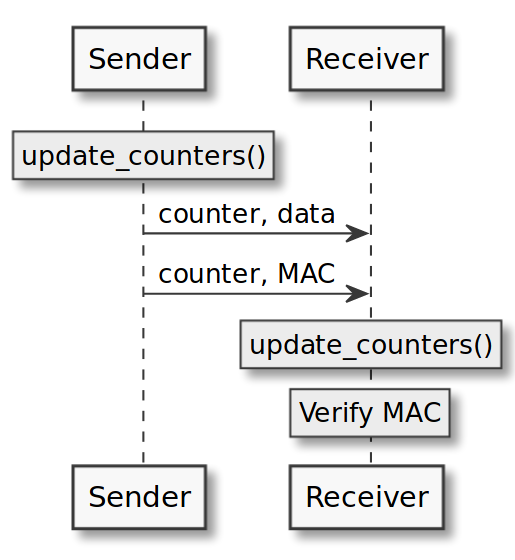
\includegraphics[width=0.6\linewidth]{Figures/LeiA_sending_msg.png}
	\caption[]{Sending an authenticated Message using LeiA}
	\label{fig:leia_sending_msg}
\end{figure}

Before sending an authenticated message with LeiA, first the message counter has
to be increased. Then the data and the MAC are sent over the corresponding CAN
identifier. The receivers will increse its own message counter for the
identifier and then verify the received MAC for the data. If this authentication
is successful the data is processed (see Fig. \ref{fig:leia_sending_msg}).

\begin{figure}[h]
    \centering
    \captionsetup{justification=centering}
	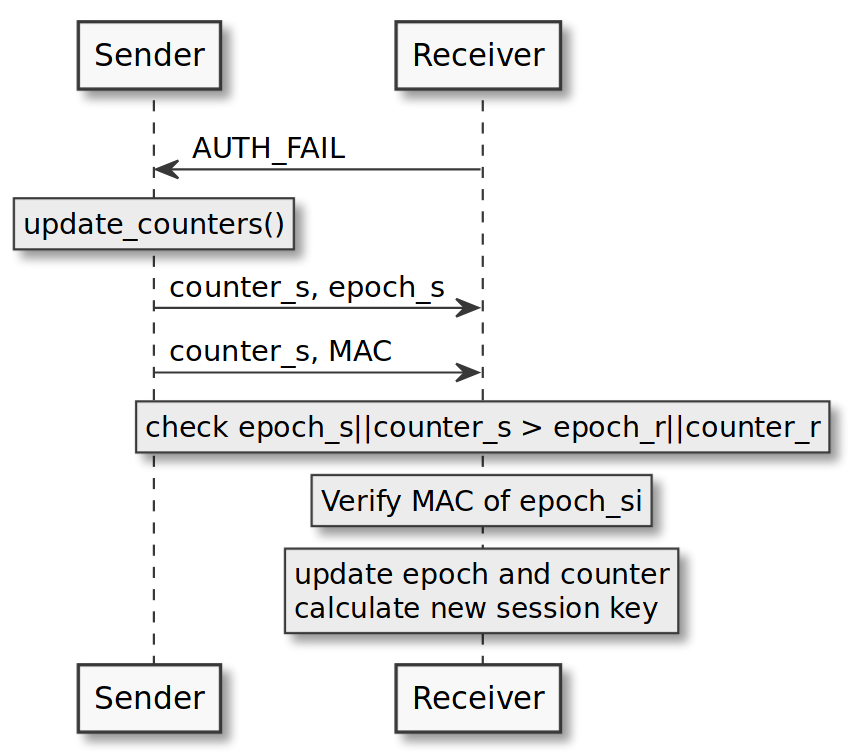
\includegraphics[width=1\linewidth]{Figures/LeiA_resync.png}
    \caption[]{Message resynchronisation after a failed message authentication 
    between Sender s and Receiver r using LeiA.}
	\label{fig:leia_resync}
\end{figure}

If the authentication of a message fail a resynchronisation between sender and
receiver is needed (see Fig. \ref{fig:leia_resync}). This means they do not use
the same session key because the epoch is out of sync. In this case the receiver
will send a AUTH\_FAIL message to signal the desynchronisation to the original
sender of the message causing the authentication problem. The sender will then
send out its current epoch value and a corresponding MAC generated from the
epoch. The receiver will accept this new epoch and counter value from the sender
if:

\begin{enumerate}
    \item The concatenated value of the received epoch and counter are higher
    than its own ($ epoch_{rec} || counter_{rec}~>~epoch_{own} || counter_{own}
    $). This check prevents replay attacks with older messages. 
    \item The provided MAC for the new epoch is successfully verified with a new
    generated session key fitting this epoch.
\end{enumerate}

Only if both conditions hold the new received value for epoch and counter are
used to update the values of the out of sync receiver. After this the sender
will resume normal sending of messages. 

In general there is a setup/initiation phase at the start. In this phase the
epoch counter will be increased and the message counter will be reset to zero.
Additionally the session keys will be generated from the long term symmetric
keys and the corresponding epoch value. After the initiation the sending of
messages can begin. Before each message the sender will update its message
counter. The receiver will update its own counter independently and then verify
the provided MAC. If there occurs an authentication error the resynchronization
procedure will be triggered. The complete outline of the protocol is given in
Figure~\ref{fig:leia_outline}.

\begin{figure}[h]
    \centering
    \captionsetup{justification=centering}
	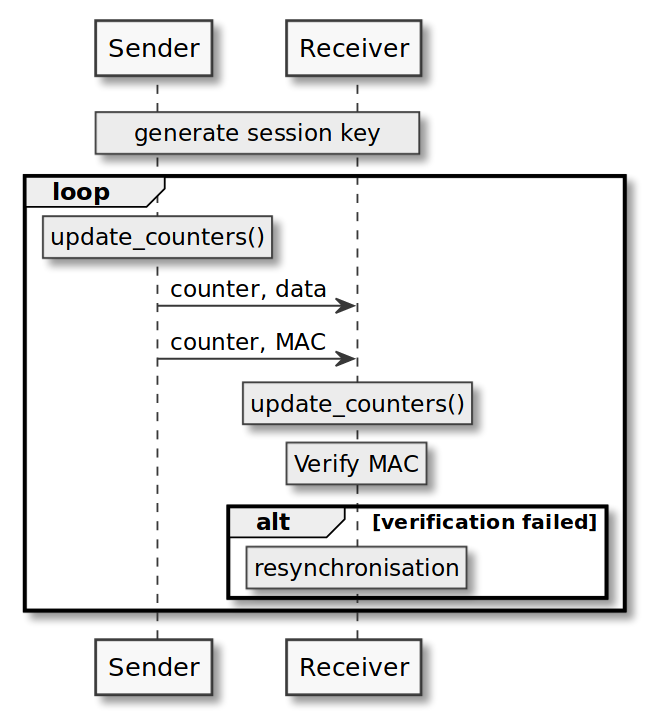
\includegraphics[width=0.9\linewidth]{Figures/LeiA_outline.png}
	\caption[]{LeiA protocol outline.}
	\label{fig:leia_outline}
\end{figure}

To be able to use an authentication protocol in the in-vehicle network
environment it needs to be lightweight. It can not introduce considerable
latency or even contain too much code because the ECUs have very limited
processing and memory capability. Therefor LeiA uses the MAC algorithm also for
generating the session keys so the code can be reused at that point. The session
keys are used for compensation of the moderate security provided by the
lightweight cryptography. So only a maximum of \( 2^16 \) messages are secured
by the same session key. After that the epoch has to change and a new session
key is used to generate the MACs. In case of a restart of the system the epoch
and thus the session key will change too. This restricts the use of a
compromised session key.

The LeiA protocol includes the counter in the extended identifier field of the
CAN message which is normally used to extend the range of possible identifiers.
The first two bits of this field are used to signal which kind of data is
included in the payload field: data, MAC of data, epoch or MAC of an epoch.
Every ECU using the LeiA protocol needs three communication channels. Therefor
it needs three different identifiers. There is a data channel, an authentication
channel and an authentication error channel. As seen in Figure
\ref{fig:leia_sending_msg}, every time data is sent there are two messages sent
out. One with the data and one with the MAC for the data. The data is sent over
the data channel and the MAC is sent over the authentication channel. The
AUTH\_FAIL messages (see Figure~\ref{fig:leia_resync}) are sent over the
authentication error channel. So every ECU broadcasting messages in the network
need to subscribe to all authentication error channels from its subscribers.

If the LeiA protocol is used like that the messages sent roughly double because
for every data message a message with a corresponding MAC is sent out. However
not all ECUs need the same level of security. So LeiA provides a scaling
mechanism by not sending out a MAC for every data message. So for every ECU it
is customizable for how many messages MACs are sent out. If there is a low
security component there could be only an authentication message sent out for
every tenth message.

In \cite{Radu2016} the authors show that the LeiA protocol is secure against
probabilistic polynomial time adversaries that can freely interact with protocol
participants meaning they have only a negligible chance of successfully
deceiving one of the participants. The protocol provides no security against
fully compromised ECUs. These possess all the keys they use to broadcast and
listen with normally. So a compromised node can listen and broadcast on all
these channels and create valid MACs for them. This is an inherent problem of
the used symmetric key cryptography. LeiA provides no security against denial of
service (DoS) attacks. But it helps by not parsing data from messages with
failed authentications.

\subsection{VatiCAN: Vetted, authenticated CAN bus}\label{subsec:vatican}

The Vetted, authenticated CAN bus protocol (VatiCAN)~\cite{Nurnberger2016} was
designed to provide maximum security while providing full backwards
compatibility to standard CAN\@. VatiCAN provides two core functionalities. The
most important functionality is of course the authentication of messages and
senders. Secondly, the protocol provides spoof detection for ECUs to detect
spoofed messages with their own identifier. Additionally the VatiCAN protocol
provides protection against replay attacks. Moreover it defines a changed CAN
arbitration to provide spoof prevention.

The authors of VatiCAN define six challenges that a CAN authentication protocol
needs to face:

\begin{enumerate}
    \item[C1] Since CAN has hard real time constraints, security mechanism for
    it can only add acceptable communication overhead not causing to
    significantly increase latency and message collisions. 
    \item[C2] Heavy-duty crypto can not be used since ECUs have very limited
    computational power and memory available.
    \item[C3] CAN messages have only a maximum payload of 8 bytes. Either the
    messages fit into these 64-bit or the data is broken up into multiple
    messages.
    \item[C4] Every vehicle must have its own cryptographic keys to not be able
    to extract working keys from another vehicle.
    \item[C5] Non-critical ECUs should not be modified to be able to keep on
    using existing hardware. So compatibility is needed with the standard CAN
    protocol.
    \item[C6] Authenticated CAN messages need to be protected against replay
    attacks without introducing a global state since CAN is a stateless
    protocol.
\end{enumerate}

VatiCAN's authors assume that an attacker does not have physical access to the
vehicle but compromised an ECU wirelessly. Furthermore they assume that the
attacker did not compromise the real target ECU\@. VatiCAN provides no security
against compromised ECUs sending authenticated messages with their own
identifiers. So the attacker needs to impersonate another ECU with the help of
the compromised one. She is also capable of reading all of the CAN messages and
learn about the other ECUs identities.

The message organization in VatiCAN uses separate messages for the
authentication. The payload of the original data message is not modified in any
way. For the authentication message the next identifier with lower priority is
used (id plus one). This assures that both, the data and the authentication
message have effectively the same priority with the authentication message
not effecting the data message. This design was chosen with challenges C1 and C5
in mind. The receipt of data messages is not influenced by the protocol and
unmodified ECUs can still read the data messages without any changes.

For message authentication (concerning C2 and C3) a lightweight key-hashed
message authentication code (HMAC) has been chosen. In particular the Keccak
algorithm standardized as SHA-3 has been used since it was shown to be the
fastest hash function on Atmel embedded microcontrollers. An input to the hash
function of 128~bit size is chosen containing the 64~bit data payload plus the
identifier for the corresponding data message and a nonce (explained below). So
this HMAC is the payload of the authentication message which is sent
additionally to the data message as described above.

The symmetric keys used in the hashing function is chosen to be of 128~bit
length and injected into the ECUs during assembly (C4). This leads to key
updates of multiple ECUs when an ECU is replaced. Gladly ECUs can normally be
upgraded through the on-board diagnostics port. So this is no problem and is
preferable to a dynamic key-agreement procedure like a Diffie-Hellman key
exchange because these are non-trivial to implement on an embedded
microcontroller.

To prevent replay attacks (C6) of any kind a nonce is used. These nonce values
need to result in different values of HMACs when used in their generation. For
every identifier a counter is used as the nonce which is incremented after every
message sent. The receiver of an HMAC needs to know the counter value to verify
the authenticity. Since the sender and its receivers can get out of sync due to
lost messages for example a sychronisation mechanism is needed. This is
accomplished by a global Nonce Generator. It periodically sends out new values
which all ECUs then use as the next counter value for their identifier after
using the current value. So the nonce / counter values are no secret and the
attacker can know them without problem. However without the secret symmetric
keys for each identifier the nonce is useless because no valid HMACs can be
computed without these keys. When two nodes get out of sync in regard to the
nonce there is a ``deaf'' time where no message can be authenticated by the
receiver until the next global nonce value is published by the Nonce Generator.
See Figure \ref{fig:vatican_deaf_time} for an overview. The authors of VatiCAN
propose an interval of 50~milliseconds for sending out global nonce values. This
would be 1\% of the bandwidth of a 500~kbit/s CAN network.

\begin{figure}[h]
    \centering
    \captionsetup{justification=centering}
	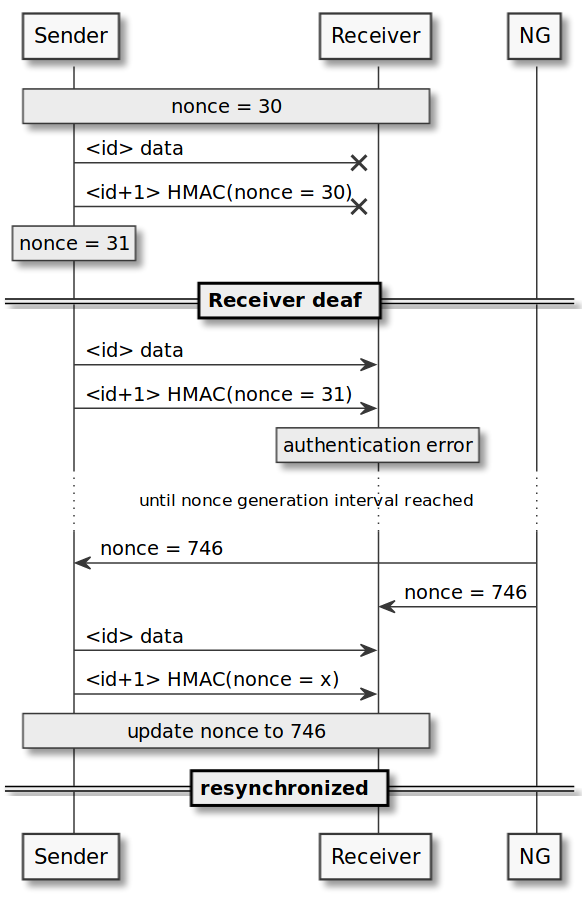
\includegraphics[width=0.8\linewidth]{Figures/VatiCAN_deaf_time.png}
	\caption[]{Nonce Generator sending out new nonce value}
	\label{fig:vatican_deaf_time}
\end{figure}

Due to the data message arriving before the authentication message, the receiver can start calculating the HMAC of the received payload. So the sender and receiver can calculate the HMAC in parallel and when the HMAC calculated by the sender is received, the receiver can directly compare the HMAC with its own calculation (See Fig.~\ref{fig:vatican_sending_msg})

\begin{figure}[h]
    \centering
    \captionsetup{justification=centering}
	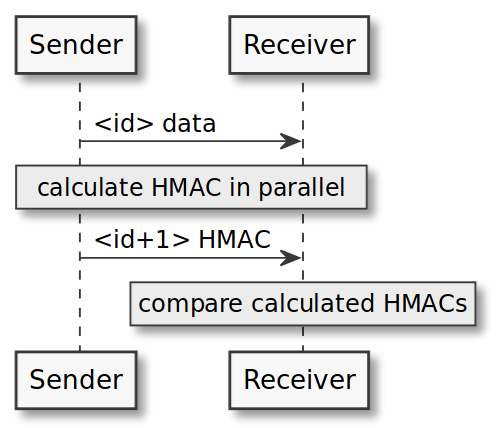
\includegraphics[width=0.8\linewidth]{Figures/VatiCAN_sending_msg.png}
	\caption[]{Sending an authenticated Message using VatiCAN}
	\label{fig:vatican_sending_msg}
\end{figure}

An ECU is easily able to identify spoofed messages of its own identifier under
the prerequisite that every ECU has its own identifier. They can simply look out
for received messages with their own identifier. If then the CRC checksum is
destroyed with dominant bits while it is sent the whole spoofed message will be
dropped by every recipient. Sadly it is not possible to destroy the CRC checksum
without modifying the CAN transceiver chip since the CRC is normally handled by
the hardware. The authors propose to use such a modified transceiver chip for
their added ECU the Nonce Generator because this component has to be added newly
anyway for VatiCAN to work. So no attacker will be possible to impersonate the
Nonce Generator and control the nonce values of the other ECUs.

The authors of VatiCAN made a Hardware-in-the-Loop-Test with an instrument
cluster, accelerator and brake pedals, ATMega microcontrollers and CAN bus
controller chips on top of a bench~\cite{Nurnberger2016}. They implemented
VatiCAN as a library for the Arduino development environment for Atmel's AVR
microcontrollers. They made a performance evaluation of their protocol and found
out that receiving an authenticated message takes 3.3~ms longer than receiving a
message without VatiCAN authentication. It was measured on an ATmega 8~bit
microcontroller which is the low end of performance for embedded boards in
vehicles. The 3.3~ms are not to be underrated. They have an impact of 0.9~m
while driving with 100~km/h on a highway.

Van Bulck et al.\ mention in \cite{VanBulck2017} that an
advanced replay attack based on the generalized birthday problem (probability
theory) is possible against the VatiCAN protocol. This is possible due to the
frequent random nonce generation. After recording only 30 minutes of traffic it
is possible to start replaying authenticated messages.